\documentclass[12pt]{beamer}
 
\usepackage[T1]{fontenc} 
\usepackage[utf8]{inputenc}
\usepackage[frenchb]{babel}
\usepackage{graphicx}
\usepackage{hyperref}

\usetheme{Warsaw}

\setbeamertemplate{navigation symbols}{}%remove navigation symbols

%\addtobeamertemplate{footline}{\insertframenumber/\inserttotalframenumber}
\defbeamertemplate*{footline}{shadow theme}
{%
  \leavevmode%
  \hbox{\begin{beamercolorbox}[wd=.5\paperwidth,ht=2.5ex,dp=1.125ex,leftskip=.3cm plus1fil,rightskip=.3cm]{author in head/foot}%
    \usebeamerfont{author in head/foot}\insertframenumber\,/\,\inserttotalframenumber\hfill\insertshortauthor
  \end{beamercolorbox}%
  \begin{beamercolorbox}[wd=.5\paperwidth,ht=2.5ex,dp=1.125ex,leftskip=.3cm,rightskip=.3cm plus1fil]{title in head/foot}%
    \usebeamerfont{title in head/foot}\insertshorttitle%
  \end{beamercolorbox}}%
  \vskip0pt%
}

% contenu de la page de titre
\title{Web des données, web sémantique}
\subtitle{Présentation du projet}
\author{Couillerot Carol, Mahier Loïc et Phalavandishvili Demetre}\institute{Faculté des Sciences et Techniques de Nantes}
\date{Année universitaire 2017/2018}
\logo{
\includegraphics[height=1.5cm]{picture/univNantes.jpg}}
	
%%%%%%%%%%%%%%%%%%%%%%%%%%%%%%%%%%%%%%%%%%%%%%%%%%%%%%%
%%%%%%%%%%%%%%%%%%%%%%%%%%%%%%%%%%%%%%%%%%%%%%%%%%%%%%%


\begin{document}

	\begin{frame}
	
		\maketitle
		
	\end{frame}

	
	\begin{frame}
	
		\frametitle{Sommaire}
   	
   		\tableofcontents[currentsubsection,sectionstyle=show/shaded,subsectionstyle=show/shaded/hide]
	
	\end{frame} 

	
	\section{Introduction}
	
		\begin{frame}
		
			\frametitle{Introduction}
		
			L’objectif du projet est de transformer les données ouvertes de l'Enseignement supérieur, de la Recherche et de l'Innovation (\url{https://data.esr.gouv.fr/FR/}) en données sémantiques et de lier ces données sémantiques au cloud.
				
		\end{frame}


	\section{Présentation des données}
	
		\begin{frame}
		
			\frametitle{Présentation des données}
		
			\centering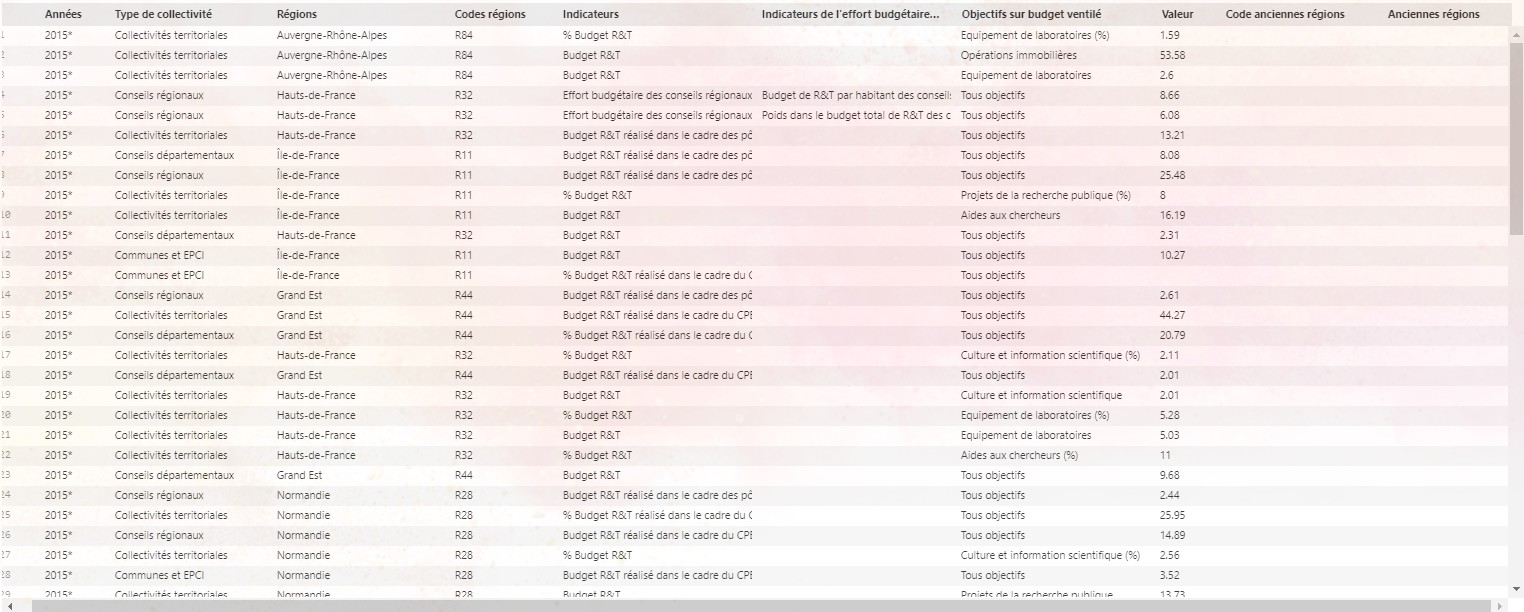
\includegraphics[height=4.5cm]{picture/data.jpg}
				
		\end{frame}
		
		
	\section{Sémantification des données}
	
		\begin{frame}
			
			\frametitle{Sémantification des données}
					
			\centering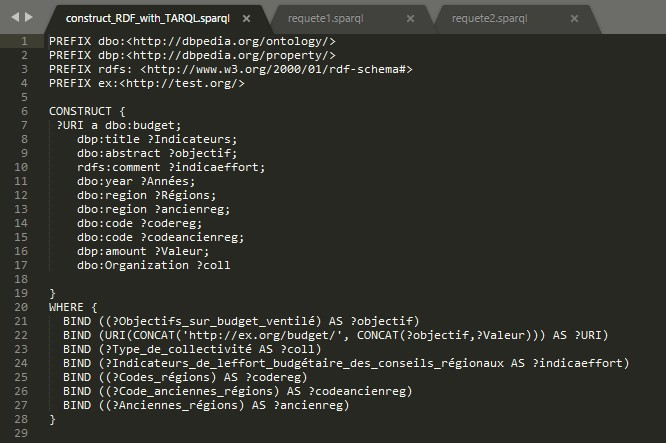
\includegraphics[height=5cm]{picture/construct.jpg}
				
		\end{frame}
		
	\section{Requêtes}
	
		\subsection{Requête 1.1}
		
			\begin{frame}
				
				\frametitle{Requête 1.1}
				
				\centering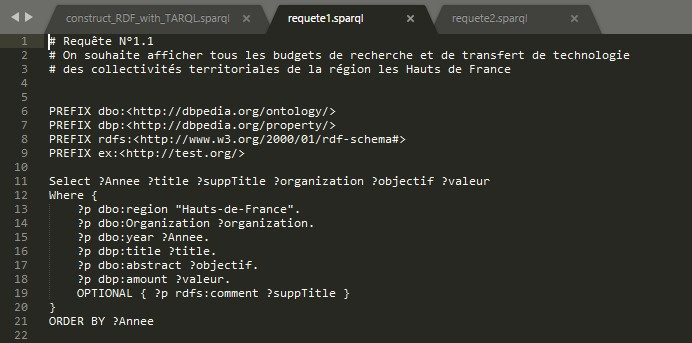
\includegraphics[height=4cm]{picture/requete11.jpg}
					
			\end{frame}		
	

		\subsection{Requête 1.2}
		
			\begin{frame}
				
				\frametitle{Requête 1.}
				
				\centering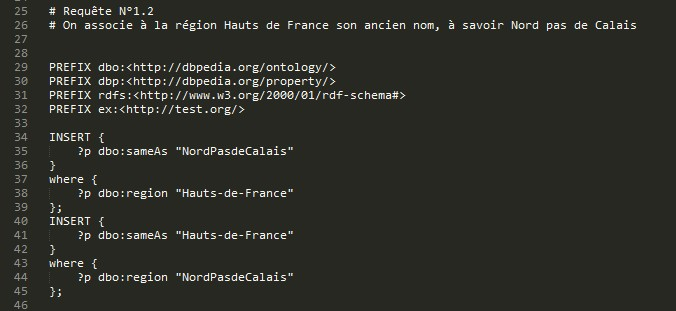
\includegraphics[height=4cm]{picture/requete12.jpg}
					
			\end{frame}	
			

		\subsection{Requête 1.3}
		
			\begin{frame}
				
				\frametitle{Requête 1.3}
				
				\centering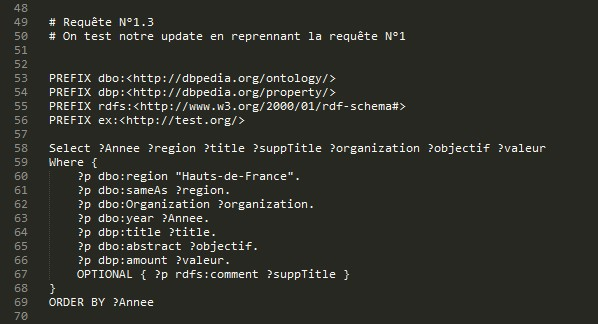
\includegraphics[height=4cm]{picture/requete13.jpg}
					
			\end{frame}	
			
							
		\subsection{Requête 2}
		
			\begin{frame}
				
				\frametitle{Requête 2}
				
				\centering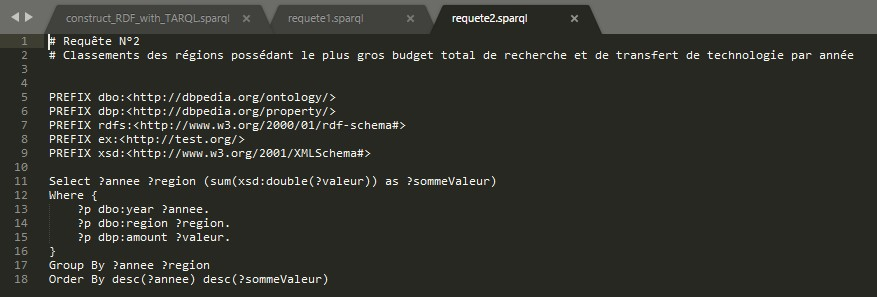
\includegraphics[height=3.5cm]{picture/requete2.jpg}
								
			\end{frame}	
			

	\section{Cloud}
	
		\begin{frame}
				
			\frametitle{Cloud}
					
		\end{frame}	


	\section{Requête cloud}
	
		\begin{frame}
				
			\frametitle{Requête cloud}
					
		\end{frame}				
										
\end{document}